%----------------------------------------------------------------------------------------
%	PACKAGES AND OTHER DOCUMENT CONFIGURATIONS
%----------------------------------------------------------------------------------------

\documentclass[final,hyperref={pdfpagelabels=false}]{beamer}

\usepackage[orientation=landscape,paperwidth=48in, paperheight=36in,scale=1.4]{beamerposter} % Use the beamerposter package for laying out the poster with a portrait orientation and an a0 paper size

\usetheme{BHK} % Use the I6pd2 theme supplied with this template
\usepackage{tikz}
\usepackage{graphicx}
\usetikzlibrary{shapes,arrows}
\usepackage{biblatex}
\bibliography{sample.bib}
\usepackage[english]{babel} % English language/hyphenation

\usepackage{amsmath, amsthm, amssymb} % For including math equations, theorems, symbols, etc
\usepackage{unicode-math}

%\usepackage{times}\usefonttheme{professionalfonts}  % Uncomment to use Times as the main font
%\usefonttheme[onlymath]{serif} % Uncomment to use a Serif font within math environments

\boldmath % Use bold for everything within the math environment

\usepackage{booktabs} % Top and bottom rules for tables

\graphicspath{{figures/}} % Location of the graphics files

\usecaptiontemplate{\small\structure{\insertcaptionname~\insertcaptionnumber: }\insertcaption} % A fix for figure numbering
\DeclareMathOperator*{\argmin}{arg\,min}

%----------------------------------------------------------------------------------------
%	TITLE SECTION 
%----------------------------------------------------------------------------------------
\title{\huge Barcode Deconvolution via Wiener Filter and Dictionary Analysis of Barcode Subsections } % Poster title

\author{Bohyun Kim, Yifei Lou, Ernie Esser} % Author(s)

\institute{Department of Mathematics, University of California, Irvine} % Institution(s)
%----------------------------------------------------------------------------------------
%	FOOTER TEXT
%----------------------------------------------------------------------------------------

\newcommand{\leftfoot}{}%http://www.LaTeXTemplates.com} % Left footer text

\newcommand{\rightfoot}{bohyunk@uci.edu} % Right footer text

%----------------------------------------------------------------------------------------

\begin{document}

\addtobeamertemplate{block end}{}{\vspace*{2ex}} % White space under blocks

\begin{frame}[t] % The whole poster is enclosed in one beamer frame

\begin{columns}[t] % The whole poster consists of two major columns, each of which can be subdivided further with another \begin{columns} block - the [t] argument aligns each column's content to the top

\begin{column}{.015\textwidth}\end{column} % Empty spacer column

\begin{column}{.3133\textwidth} % The first column

%----------------------------------------------------------------------------------------
%	MOTIVATION
%----------------------------------------------------------------------------------------

\begin{block}{\Large Motivation}
\vskip-0.4em
While current barcode decoding systems provide reliable results in correctly reading barcodes at a close range, we want to increase the limits of these systems, so they will be able to read these codes with extreme levels of blur and noise. Building off of the work ``Non-Blind Barcode Deconvolution by Gradient Projection [2]'', we propose a method to analyze a subsection of a barcode with an unknown signal and blurring function(\textbf{Blind Deconvolution}). %This function uses the \textbf{Wiener Filter} to analyze and filter out noise and blur from a blurry barcode, while using a dictionary brute force method to try every possible combination of the first two digits of a barcode to find a blurring function and clean signal that created the original input. Through testing, our method successfully analyzes a subsection of a blurry barcode and returns a fragment of a clean barcode along with a kernel estimate similar to the actual function that blurred the image, possibly allowing future processes to accept even more limited data and correctly reconstruct the original data.

\end{block}

%----------------------------------------------------------------------------------------
%	PROBLEM SETTING
%----------------------------------------------------------------------------------------

\begin{block}{\Large Problem Setting}
\vskip-0.5em
\begin{itemize}
\item Barcode Structure
\end{itemize}

\begin{figure}
\centering
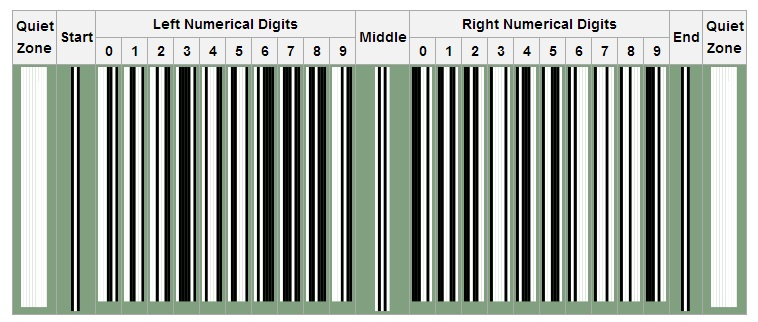
\includegraphics[clip,trim=0 0 2.5in 1.25in, scale=0.85]{barcode_structure.jpg}
\caption{UPC-A type Barcode Structure}
\end{figure}

\vskip-0.7em
\begin{itemize}
\item Image Degradation Model
\end{itemize}

\vskip-1.6em
\begin{equation}
\label{convolution}
\Large f=k*u+n
\end{equation}
Where a $f$ represents blurred barcode, $u$ represents an uncorrupted barcode, $k$ represents a blurring kernel, $n$ represents a random noise, and * represents the convolution operator.


\end{block}

%----------------------------------------------------------------------------------------
%	METHODS;IN SUMMARY
%----------------------------------------------------------------------------------------

\begin{block}{\Large Methods: In Summary}
\vskip 0.3em
\begin{center}
%define the style of the diagram
\tikzstyle{decision} = [diamond, draw, fill=red!50, text width=2.9em, text centered, node distance=0.5cm, inner sep=0pt]
\tikzstyle{block} = [rectangle, draw, fill=green!50, text width=2.4em, text centered, rounded corners, minimum height=0.4em]
\tikzstyle{block2} = [rectangle, draw, fill=blue!35, text width=2.4em, text centered, rounded corners, minimum height=0.4em]
\tikzstyle{line} = [draw, -latex']
\tikzstyle{cloud} = [draw, ellipse,fill=blue!35, text width=1.48em, text centered,  node distance=1.5em, minimum height=0.3em]
\tikzstyle{dot} = [rectangle, fill = white, text width = 2em, text centered, rounded corners, minimum height = 0.5em]
\tikzstyle{final} = [ellipse, draw, fill=yellow!50, text width=1.3em, text centered, rounded corners, minimum height=0.5em]


%Drawing Diagram
\begin{figure}
\begin{tikzpicture}[node distance = 3em, auto]

%Drawing Blocks
\node[block](u00){\small Use\\ $u_{00}$};
\node[block, below of = u00 ](u01){\small Use\\ $u_{01}$};
\node[block, below of = u01](u02){\small Use\\ $u_{02}$};
\node[block2, left of = u01, node distance = 3.9em](f){\small Let\\ first 17 digits\\ as\\ $f$};
\node[block, right of = u00, node distance = 3.9em](k00){\small Find\\ $k_{00}$};
\node[block, right of = u01, node distance = 3.9em](k01){\small Find\\ $k_{01}$};
\node[block, right of = u02, node distance = 3.9em](k02){\small Find\\ $k_{02}$};
\node[block, right of = k00, node distance = 3.9em](e00){\small Calculate $e_{00}$};
\node[block, right of = k01, node distance = 3.9em](e01){\small Calculate $e_{01}$};
\node[block, right of = k02, node distance = 3.9em](e02){\small Calculate $e_{02}$};
\node[decision, right of = e01, node distance = 4.8em](decision){\small Find $min(e_{ij})$};
\node[final, right of = decision, node distance = 4.5em](final){\small Final\\ $k$ and $u$};
%
\node[dot, below of = u02](dotk0){\small $\vdots$};
\node[dot, below of = k02](dotk1){\small $\vdots$};
\node[dot, below of = e02](dotk2){\small $\vdots$};
%
%%Draw paths
\path[line](f) |-(u00);
\path[line](f) -- (u01);
\path[line](f) |- (u02);
\path[line](u00) --(k00);
\path[line](u01) --(k01);
\path[line](u02) --(k02);
\path[line](k00) --(e00);
\path[line](k01) --(e01);
\path[line](k02) --(e02);
\path[line, dashed](f) |- (dotk0);
\path[line](e00) -| (decision);
\path[line](e01) -- (decision);
\path[line](e02) -| (decision);
\path[line, dashed](dotk2) -| (decision);
\path[line](decision) -- (final);

\end{tikzpicture}
%\caption{Our method in summary}
\label{tikz}
\end{figure}
\end{center}

\vskip -0.4em
\end{block}
\end{column} %end of first column


%----------------------------------------------------------------------------------------
%	METHODS; IN DEPTH
%----------------------------------------------------------------------------------------
\begin{column}{.015\textwidth}\end{column} % Empty spacer column
\begin{column}{.3133\textwidth}
\begin{block}{\Large Methods: In Depth}
\vskip-0.4em
We assume each portion of signal is convoluted in the same way and follow through each step from 00$\sim$99
\vskip-0.1em
\begin{itemize}
\item Estimate $k$ and $u$ 
\begin{itemize}
\item Roughly estimate $k$ and $u$ from $\underset{K,u}{\mathrm{\text{arg min}}}(||Ku - f||^2 + \lambda||u||^2)$ by Wiener Filter
\item Refine $k$ using Gradient Descent 
\end{itemize}

\item Calculate error for each $k$ and $u$ 
\begin{itemize}
\item Calculate $e = |Ku-f|$ 
\end{itemize}
\end{itemize}
\vskip-0.4em
After calculating each error, choose $k$ and $u$ such that they minimize $e$. Use the $k$ in order to decode other sequences.
\end{block}

%----------------------------------------------------------------------------------------
%	METHODS: IN FIGURE
%----------------------------------------------------------------------------------------

\begin{block}{\Large Methods: In Figure}

\begin{itemize}
\item Inaccurate estimation
\end{itemize}
\vskip-0.5em

\begin{column}{.45\textwidth}
	\begin{figure}[!htb]
	\centering
	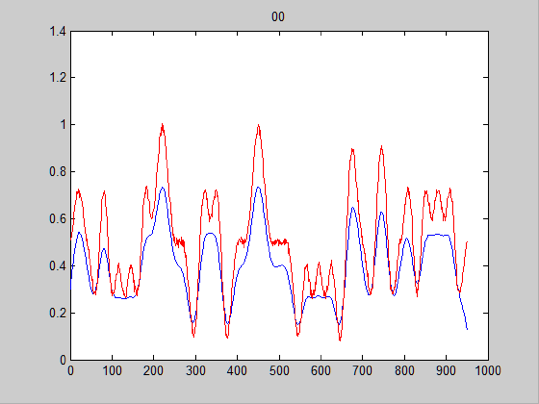
\includegraphics[width=0.98\linewidth]{u00.png}
	\caption{\hskip-0.4em Convoluted barcode for 00($u00$)}
	\end{figure}
\end{column}
\begin{column}{.08\textwidth}\end{column}
\begin{column}{.45\textwidth}
	\begin{figure}[!htb]
	\centering
	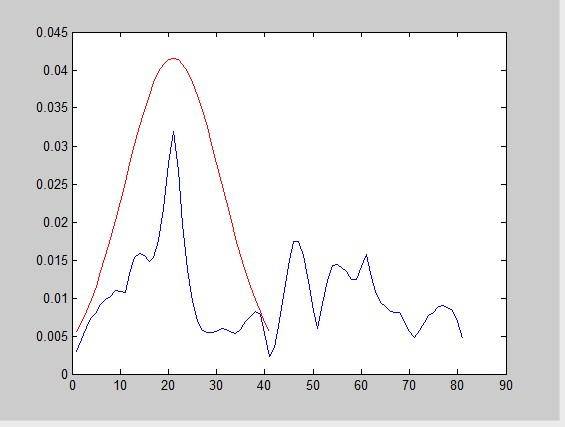
\includegraphics[width=0.98\linewidth]{k00.jpeg}
	\caption{Kernel for 00($k00$)}
	\end{figure}
\end{column}
\vspace{1.5em}
\begin{itemize}
\item Accurate estimation
\end{itemize}
\vskip-0.5em

\begin{column}{.45\textwidth}
	\begin{figure}[!htb]
	\centering
	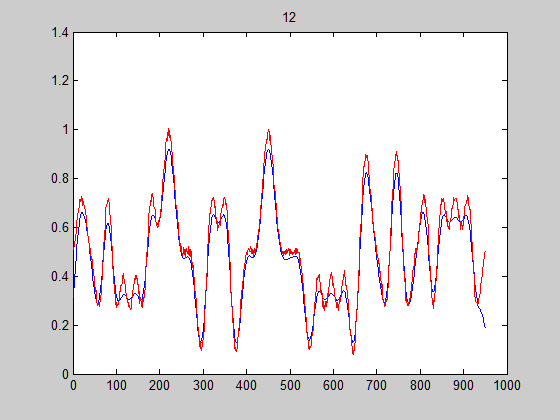
\includegraphics[width=0.98\linewidth]{u12.png}
	\caption{\hskip-0.4em Convoluted barcode for 12($u12$)}
	\end{figure}
\end{column}
\begin{column}{.45\textwidth}
	\begin{figure}[!htb]
	\centering
	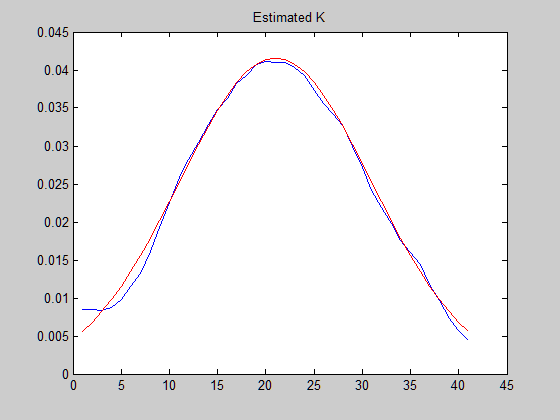
\includegraphics[width=0.98\linewidth]{k12.png}
	\caption{Kernel for 12($k12$)}
	\end{figure}
\end{column}

\end{block}


%----------------------------------------------------------------------------------------

\end{column} % End of the second column

 

%----------------------------------------------------------------------------------------
%	MODEL VALIDATION
%----------------------------------------------------------------------------------------
\begin{column}{.015\textwidth}\end{column} % Empty spacer column
\begin{column}{.3133\textwidth} % The third column

\begin{block}{\Large Model Validation}
	\vskip-0.2em
	\begin{figure}[!htb]
	\centering
	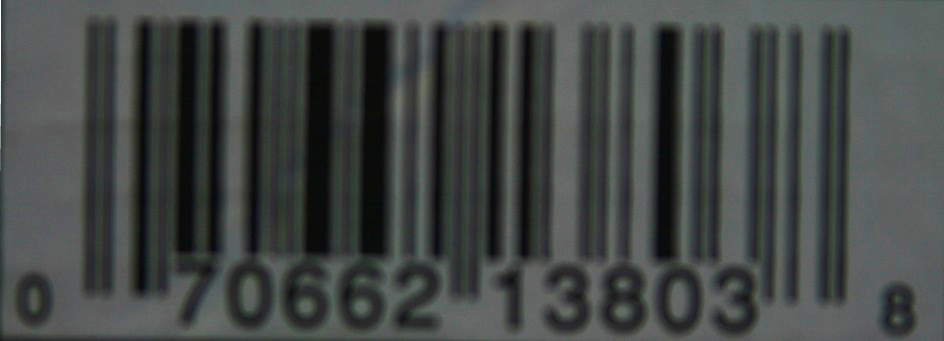
\includegraphics[width=0.5\linewidth]{ramen.png}
	\vskip-0.8em
	\caption{Blurred barcode}
	\end{figure}
	
	\vskip-0.4em
	\begin{figure}[!htb]
	\centering
	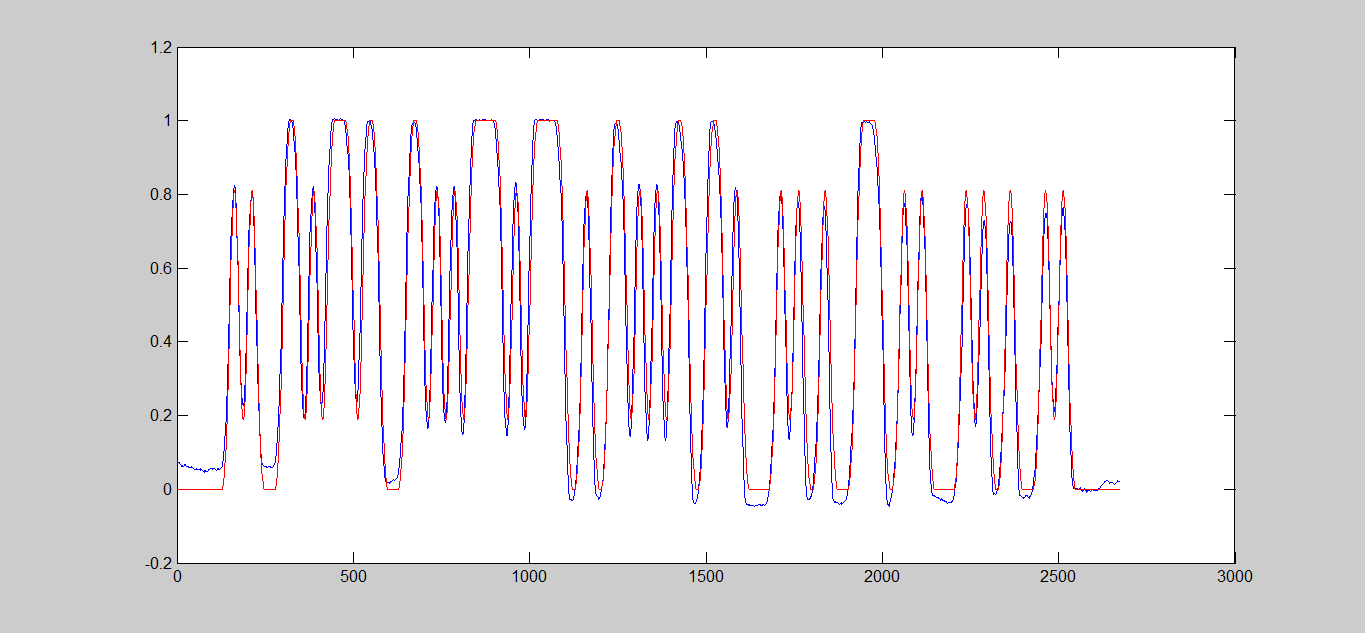
\includegraphics[width=0.9\linewidth]{comparison.png}
	\vskip-0.8em
	\caption{Barcode analysis}
	\end{figure}
	\vskip-0.8em

\end{block}
\vskip-0.3em
%------------------------------------------------

%----------------------------------------------------------------------------------------
%	CONCLUSION
%----------------------------------------------------------------------------------------

\begin{block}{\Large Model Validation}
\vskip-0.7em
\begin{itemize}
\item We successfully deconvoluted a barcode with extreme blur and noise.
\vskip-0.8em
\item We established a process of blind deconvolution for barcodes
\vskip-0.8em
\item We plan to refine our process to function over wider range of blur and noise.
\vskip-0.8em
\end{itemize}
\vskip-0.4em

\end{block}

\vskip-0.3em
%----------------------------------------------------------------------------------------
%	REFERENCES
%----------------------------------------------------------------------------------------

\begin{block}{\Large References}

\vskip-0.2em
\normalsize{
[1] Rustum Choksi and Yves van Gennip. Deblurring of one dimensional bar codes via total variation energy minimization. \emph{SIAM Journal on Imaging Sciences}, 2010.

[2] Christine Lew and Dheyani Malde. Non-blind barcode deconvolution by gradient projection. iCamp 2012 Barcode group, 2012.

[3] Fadil Santosa Mark A. Iwen and Rachel Ward. A symbol-based algorithm for decoding bar codes. \emph{SIAM Journal on Imaging Sciences}, 2013.}

\end{block}

%----------------------------------------------------------------------------------------
%	ACKNOWLEDGEMENTS
%----------------------------------------------------------------------------------------

\vskip-0.4em

\begin{block}{\Large Acknowledgments}
\vskip-0.3em
A great appreciation to Interdisciplinary Computational and Applied Mathematics Program(iCAMP) in UCI and my advisors Yifei Lou and Ernie Esser.

\end{block}

%----------------------------------------------------------------------------------------
%	CONTACT INFORMATION
%----------------------------------------------------------------------------------------

%----------------------------------------------------------------------------------------

\end{column} % End of the second column

\begin{column}{.015\textwidth}\end{column} % Empty spacer column

\end{columns} % End of all the columns in the poster

\end{frame} % End of the enclosing frame

\end{document}